%!TEX root = ../dissertation.tex
\begin{savequote}[75mm]
Nulla facilisi. In vel sem. Morbi id urna in diam dignissim feugiat. Proin molestie tortor eu velit. Aliquam erat volutpat. Nullam ultrices, diam tempus vulputate egestas, eros pede varius leo.
\qauthor{Quoteauthor Lastname}
\end{savequote}

\chapter{The title of chapter one}

\newthought{There's something to be said} for having a good opening line. Morbi commodo, ipsum sed pharetra gravida, orci  $x = 1/\alpha$ magna rhoncus neque, id pulvinar odio lorem non turpis. Nullam sit amet enim. Suspendisse id velit vitae ligula volutpat condimentum. Aliquam erat volutpat. Sed quis velit. Nulla facilisi. Nulla libero. Vivamus pharetra posuere sapien. Nam consectetuer. Sed aliquam, nunc eget euismod ullamcorper, lectus nunc ullamcorper orci, fermentum bibendum enim nibh eget ipsum. Donec porttitor ligula eu dolor. Maecenas vitae nulla consequat libero cursus venenatis. Nam magna enim, accumsan eu, blandit sed, blandit a, eros.
$$\zeta = \frac{1039}{\pi}$$

% For an example of a full page figure, see Fig.~\ref{fig:myFullPageFigure}.

Lorem ipsum dolor sit amet, consectetuer adipiscing elit. Morbi commodo, ipsum sed pharetra gravida, orci magna rhoncus neque, id pulvinar odio lorem non turpis. Nullam sit amet enim. Suspendisse id velit vitae ligula volutpat condimentum. Aliquam erat volutpat. Sed quis velit. Nulla facilisi. Nulla libero. Vivamus pharetra posuere sapien. Nam consectetuer. Sed aliquam, nunc eget euismod ullamcorper, lectus nunc ullamcorper orci, fermentum bibendum enim nibh eget ipsum. Donec porttitor ligula eu dolor. Maecenas vitae nulla consequat libero cursus venenatis. Nam magna enim, accumsan eu, blandit sed, blandit a, eros.

\texttt{This is a line of code.}

Lorem ipsum dolor sit amet, consectetuer adipiscing elit. Morbi commodo, ipsum sed pharetra gravida, orci magna rhoncus neque, id pulvinar odio lorem non turpis. Nullam sit amet enim. Suspendisse id velit vitae ligula volutpat condimentum. Aliquam erat volutpat. Sed quis velit. Nulla facilisi. Nulla libero. Vivamus pharetra posuere sapien. Nam consectetuer. Sed aliquam, nunc eget euismod ullamcorper, lectus nunc ullamcorper orci, fermentum bibendum enim nibh eget ipsum. Donec porttitor ligula eu dolor. Maecenas vitae nulla consequat libero cursus venenatis. Nam magna enim, accumsan eu, blandit sed, blandit a, eros.


\begin{figure}
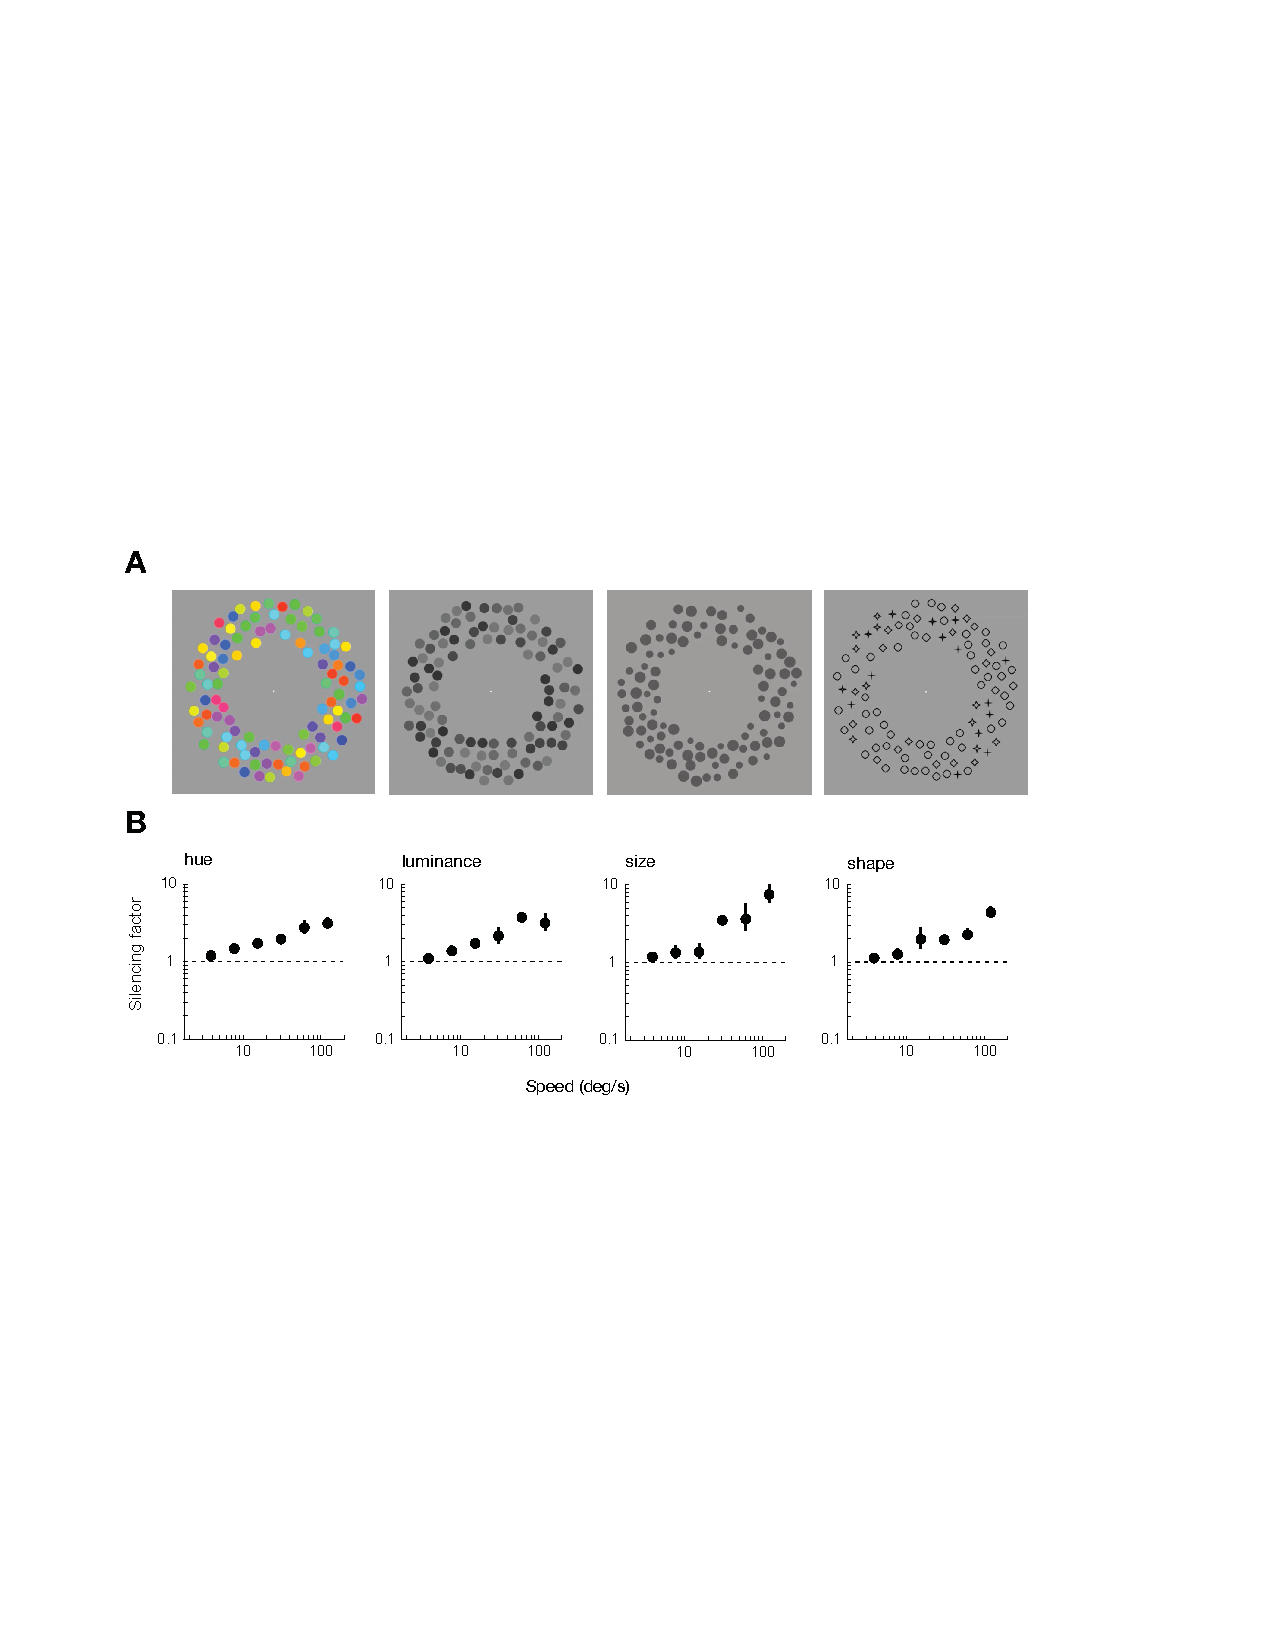
\includegraphics[width=\textwidth]{figures/fig1}
\caption[Short figure name.]{This is a figure that floats inline and here is its caption.
\label{fig:myInlineFigure}}
\end{figure}

Pellentesque vel dui sed orci faucibus iaculis. Suspendisse dictum magna id purus tincidunt rutrum. Nulla congue. Vivamus sit amet lorem posuere dui vulputate ornare. Phasellus mattis sollicitudin ligula. Duis dignissim felis et urna. Integer adipiscing congue metus. Nam pede. Etiam non wisi. Sed accumsan dolor ac augue. Pellentesque eget lectus. Aliquam nec dolor nec tellus ornare venenatis. Nullam blandit placerat sem. Curabitur quis ipsum. Mauris nisl tellus, aliquet eu, suscipit eu, ullamcorper quis, magna. Mauris elementum, pede at sodales vestibulum, nulla tortor congue massa, quis pellentesque odio dui id est. Cras faucibus augue.

%% Requires fltpage2 package
%%
% \begin{FPfigure}
% 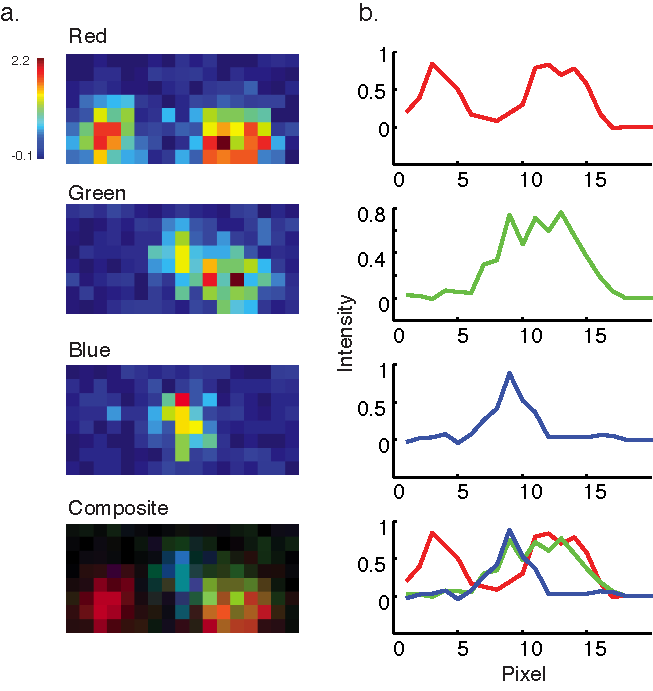
\includegraphics[width=\textwidth]{figures/fullpage}
% \caption[Short figure name.]{This is a full page figure using the FPfigure command. It takes up the whole page and the caption appears on the preceding page. Its useful for large figures. Harvard's rules about full page figures are tricky, but you don't have to worry about it because we took care of it for you. For example, the full figure is supposed to have a title in the same style as the caption but without the actual caption. The caption is supposed to appear alone on the preceding page with no other text. You do't have to worry about any of that. We have modified the fltpage package to make it work. This is a lengthy caption and it clearly would not fit on the same page as the figure. Note that you should only use the FPfigure command in instances where the figure really is too large. If the figure is small enough to fit by the caption than it does not produce the desired effect. Good luck with your thesis. I have to keep writing this to make the caption really long. LaTex is a lot of fun. You will enjoy working with it. Good luck on your post doctoral life! I am looking forward to mine. \label{fig:myFullPageFigure}}
% \end{FPfigure}
% \afterpage{\clearpage}

Suspendisse vestibulum dignissim quam. Integer vel augue. Phasellus nulla purus, interdum ac, venenatis non, varius rutrum, leo. Pellentesque habitant morbi tristique senectus et netus et malesuada fames ac turpis egestas. Duis a eros. Class aptent taciti sociosqu ad litora torquent per conubia nostra, per inceptos hymenaeos. Fusce magna mi, porttitor quis, convallis eget, sodales ac, urna. Phasellus luctus venenatis magna. Vivamus eget lacus. Nunc tincidunt convallis tortor. Duis eros mi, dictum vel, fringilla sit amet, fermentum id, sem. Phasellus nunc enim, faucibus ut, laoreet in, consequat id, metus. Vivamus dignissim. Cras lobortis tempor velit. Phasellus nec diam ac nisl lacinia tristique. Nullam nec metus id mi dictum dignissim. Nullam quis wisi non sem lobortis condimentum. Phasellus pulvinar, nulla non aliquam eleifend, tortor wisi scelerisque felis, in sollicitudin arcu ante lacinia leo.
